\documentclass[12pt]{report}
\usepackage{graphicx}
\usepackage[utf8]{vietnam}
\usepackage[left=3cm, right=3cm, top=3cm, bottom =3cm]{geometry}
\usepackage{pdfpages}
\usepackage{fancyhdr}
\usepackage{hyperref}
\usepackage{etoolbox}

% \setcounter{tocdepth}{4}

% Link color setup
\hypersetup{
	colorlinks = true,
	linkcolor = black,
	citecolor = blue
}

% Change format of page
\pagestyle{fancy}
\fancyhf{}
\fancyhead{}
\fancyfoot{}
\fancyhead[L]{Hệ điều hành}
\fancyfoot[L]{Tạ Quang Tùng -- MSSV: 20154280 -- Lớp: KSTN-CNTT-K60}
\fancyfoot[R]{\thepage}
\renewcommand{\headrulewidth}{1pt}
\renewcommand{\footrulewidth}{1pt}

\patchcmd{\chapter}{\thispagestyle{plain}}{\thispagestyle{fancy}}{}{}

\renewcommand{\thesection}{\arabic{section}}
\renewcommand{\thesubsection}{\thesection.\arabic{subsection}}

% format
\usepackage{titlesec}
\usepackage{etoolbox}
\makeatletter
\patchcmd{\ttlh@hang}{\parindent\z@}{\parindent\z@\leavevmode}{}{}
\patchcmd{\ttlh@hang}{\noindent}{}{}{}
\makeatother

\titleformat{\subsection}
{\normalfont\large\bfseries}{\thesubsection}{1em}{}
\titleformat{\subsubsection}
{\normalfont\normalsize\sffamily\bfseries}{\thesubsubsection}{1em}{}

\usepackage{listings}
\usepackage{color}

\lstdefinestyle{customc}{
  belowcaptionskip=1\baselineskip,
  breaklines=true,
  frame=L,
  xleftmargin=\parindent,
  language=C++,
  showstringspaces=false,
  basicstyle=\footnotesize\ttfamily\color{black},
  keywordstyle=\bfseries\color{blue!40!black},
  commentstyle=\itshape\color{purple!40!black},
  identifierstyle=\color{black},
  stringstyle=\color{orange},
}
\lstset{escapechar=@, style=customc}

\begin{document}

\vspace*{5cm}
\begin{LARGE}
\sffamily
\bfseries
\begin{center}
BÁO CÁO \\
CƠ CHẾ PHÂN ĐOẠN, PHÂN TRANG \\ 
TRONG HỌ VI XỬ LÝ INTEL X86
\end{center}
\end{LARGE}

\vspace*{2cm}
\begin{large}
\sffamily\bfseries
\begin{center}
Sinh viên thực hiện: Tạ Quang Tùng \\
MSSV: 20154280 \\
Lớp: KSTN-CNTT-K60
\end{center}
\end{large}

\newpage
\tableofcontents

\newpage

\section{Protection Ring - Cơ chế bảo vệ của x86}
Trong khoa học máy tính, cơ chế bảo vệ phân cấp (hay còn gọi là protection ring) là cơ chế bảo vệ những dữ liệu, những chức năng khỏi việc bị hỏng hóc (tăng khả năng chịu lỗi của hệ thống) hay bởi những hành độc, tác nhân độc hại (tăng tính bảo mật). \cite{protection_ring}  

Các hệ điều hành máy tính cung cấp các mức truy cập khác nhau tới tài nguyên. Một protection ring là một trong hai hay nhiều lớp đặc quyền đối với một hệ thống máy tính. 
\begin{figure}[h]
\centering
\caption{Protection Ring trong họ Intel x86}
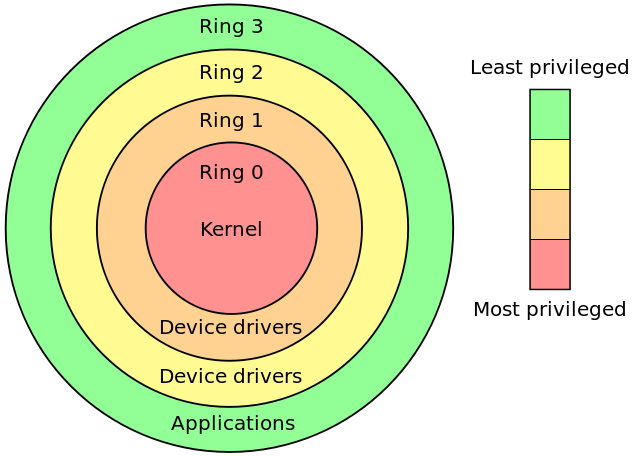
\includegraphics[width=5cm]{protection_ring.png}
\end{figure}

Trong họ vi xử lý x86, có tổng cộng 4 mức đặc quyền, được đánh số từ 0 cho đến 3. Mức 0 là mức có đặc quyền cao nhất. Nhưng hầu hết các nhân hệ điều hành cho x86 như Windows, Linux chỉ sử dụng hai mức đặc quyền là mức 0 và mức 3. Hai mức 0 và 3 đó thường được gọi lần lượt là kernel mode và user mode. Kernel mode chỉ được sử dụng bởi nhân (kernel) của hệ điều hành, còn user mode chủ yếu trong thời gian hoạt động của các tiến trình thông thường.

Có khoảng 15 instruction (lệnh của CPU), chỉ được sử dụng ở mức đặc quyền 0 của CPU \cite{x86-rings}. Có nhiều những instruction khác thì bị giới hạn  trong các toán hạng của nó khi ở ngoài mức 0. Những instruction chỉ được sử dụng ở mức đặc quyển 0 đó có thể phá vỡ cơ chế bảo vệ hoặc gây nên xáo trộn trong hệ thống nếu được phép sử dụng ở user mode.

\section{Phân đoạn trong phần cứng x86}
Bắt đầu từ phiên bản 80286, Trong vi xử lý Intel có tồn tại hai cách để thực hiện dịch địa chỉ đó là \textit{real mode} và \textit{protected mode}. Real mode tồn tại chủ yếu để duy trì tính tương thích ngược đối với những thế hệ vi xử lý cũ và để cho phép hệ điều hành có thể khởi động. \cite{address_translation}

Trong protected mode, địa chỉ tồn tại dưới 3 dạng:
\begin{itemize}
\item Địa chỉa logic: Địa chỉ tồn tại dưới dạng \textit{segment:offset}, là địa chỉ được CPU được sử dụng bên trong, trước khi qua khối phân đoạn. 
\item Địa chỉ tuyến tính: Địa chỉ được tạo từ địa chỉ logic sau khi qua quá trình phân đoạn và trước khi qua quá trình phân trang. 
\item Địa chỉ vật lý: Là địa chỉ được truyền ra ngoài CPU tới các thành phần khác trong hệ thống (Ví dụ RAM).
\end{itemize}

\begin{figure}[h]
\centering
\caption{Quá trình dịch địa chỉ trong x86}
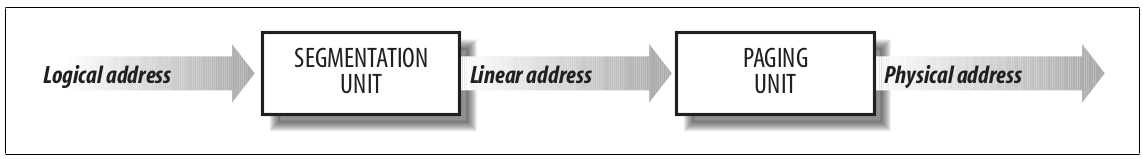
\includegraphics[width=\textwidth]{address_translation.png}
\end{figure}

\subsection{Các thanh ghi chỉ định đoạn}
Địa chỉ logic gồm hai phần \textit{segment} và \textit{offset}, phần \textit{segment} được gọi là phần chỉ định đoạn, gồm 16 bit. Được chia thành các phần như mô tả trong hình: 
\begin{figure}[h]
\centering
\caption{Định dạng của \textit{segment}}
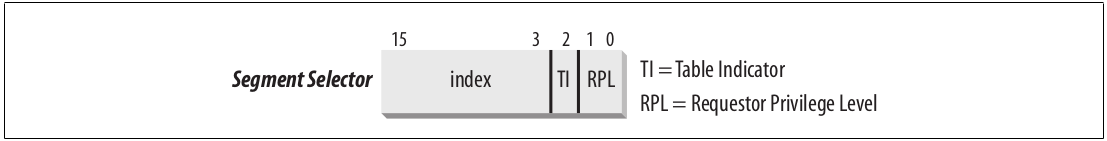
\includegraphics[width=\textwidth]{segment_selector.png}
\end{figure}

Hai thành phần chính trong cơ chế phân đoạn của x86 là các thanh ghi segment 16 bit như cs (code segment), ds (data segment), ss (stack segment),... và bảng quản lý đoạn. Có hai bảng quản lý đoạn: Global Descriptor Table (GDT) và Local Descriptor Table (LDT), nằm trong bộ nhớ chính, địa chỉ của chúng được quản lý bởi hai thanh ghi gdtr và ldtr. Bit TI trong mỗi thanh ghi segment chỉ định bảng nào sẽ được lựa chọn, bằng 0 nếu như đang sử dụng GDT, bằng 1 là LDT. Phần index là chỉ số của phần tử tương ứng nằm trong bảng quản lý đoạn. 

Mỗi phần tử trong bảng quản lý đoạn có 8 byte, được chia thành nhiều trường như sau: 
\begin{itemize}
\item Base: Chứa địa chỉ tuyến tính của byte đầu tiên trong đoạn. 
\item G - granularity flag: Gồm 1 bit; nếu nó bằng 0, kích thước của đoạn được thể hiện dưới dạng byte; ngược lại, kích thước được thể hiện dưới dạng số nguyên lần của 4096 byte. 
\item Limit: 20 bit; Giới hạn của đoạn, có thể biểu diễn $2^{10}$ giá trị, nếu G = 0 thì đoạn đó có kích thước lớn nhất là 1MB; ngược lại, đoạn có kích thước lớn nhất là 4GB.
\end{itemize}

\bibliographystyle{plain}
\bibliography{refs}
\end{document}